
\section{Ebola Paper}
\label{section:ebola_paper}
In Chritian L. Althaus's paper, the epidemiologist uses data from the Ebola spread in three different West African countries to understand the impact of the implemented control measures. To do this, the researcher needs to estimate parameters like the basic and effective reproduction number of the virus.

These parameters are estimated by doing a best fit optimization on the parameters applied to an SEIR model. The experiment is to use an ODE model with certain values of these parameters and calculate the error of these models at the real-life recorded data points. We run different ODE models by changing the parameters until we minimise these errors. The model with that minimum error is the 'best fit' model and the parameters that were used by this model are our estimates. These estimates are then used to understand the spread of the virus. 

We note that the ODE model is run inside an optimisation algorithm and thus its efficiency is critical as the algorithm will need to build several ODE models with each different set of parameters.

The following is the pseudo-code for our attempt at replicating the experiment:

\begin{minipage}{\linewidth}
\begin{lstlisting}[language=Python]
data = read_csv("ebola_data.csv")

function model(t, y, parms):
    // define the SEIR model
    return (dSdt, dEdt, dIdt, dRdt)

function ssq(parms):
    // get the model
    out = ode(model, initial_value, times, parms)

    // we calculate the error from the data points as such:
    ssq = abs(out.C - data.C) + abs(out.D - data.D)
    return ssq

parms = c(beta=0.27, f=0.74, k=0.0023)
fit = optimise(par=parms, errorFunc=ssq)

// fit will contain the optimal parameter values...
\end{lstlisting}
\end{minipage}

The figure that were reported in the paper is shown in Figure $\ref{fig:original_figure_SEIR_paper}$. Our figures are as shown in Figures $\ref{fig:my_fit_Gui}$, $\ref{fig:my_fit_SL}$ and $\ref{fig:my_fit_Lib}$

\begin{figure}[h]
	\centering
	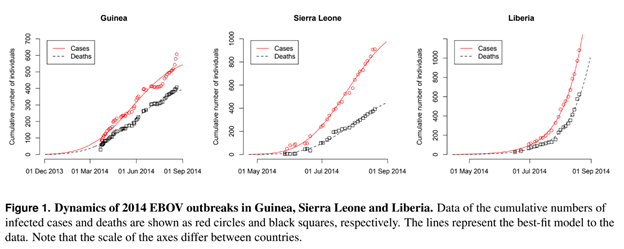
\includegraphics[width=1\linewidth]{./figures/original_figure_SEIR_paper}
	\caption{Original figure in Ebola paper}
	\label{fig:original_figure_SEIR_paper}
\end{figure}

\begin{figure}[h]
	\centering
	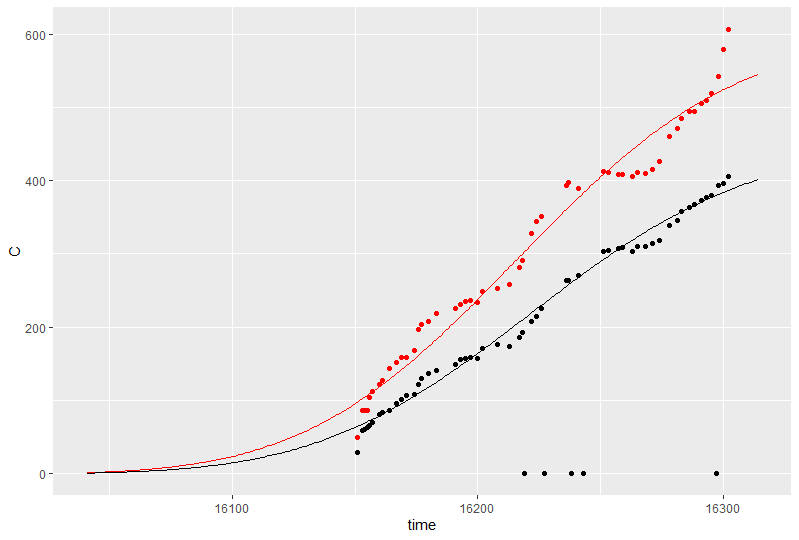
\includegraphics[width=0.7\linewidth]{./figures/my_fit_Gui}
	\caption{Our Guinea Figure}
	\label{fig:my_fit_Gui}
\end{figure}

\begin{figure}[h]
	\centering
	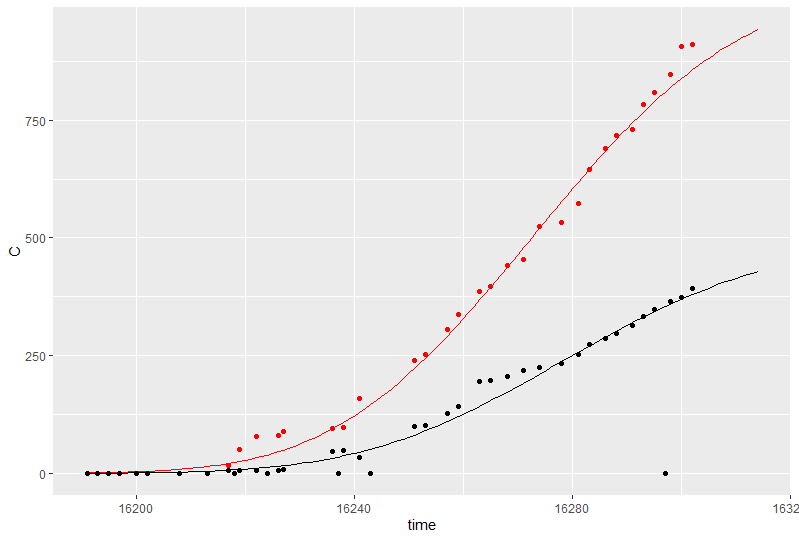
\includegraphics[width=0.7\linewidth]{./figures/my_fit_SL}
	\caption{Our Sierra Leone Figure}
	\label{fig:my_fit_SL}
\end{figure}

\begin{figure}[h]
	\centering
	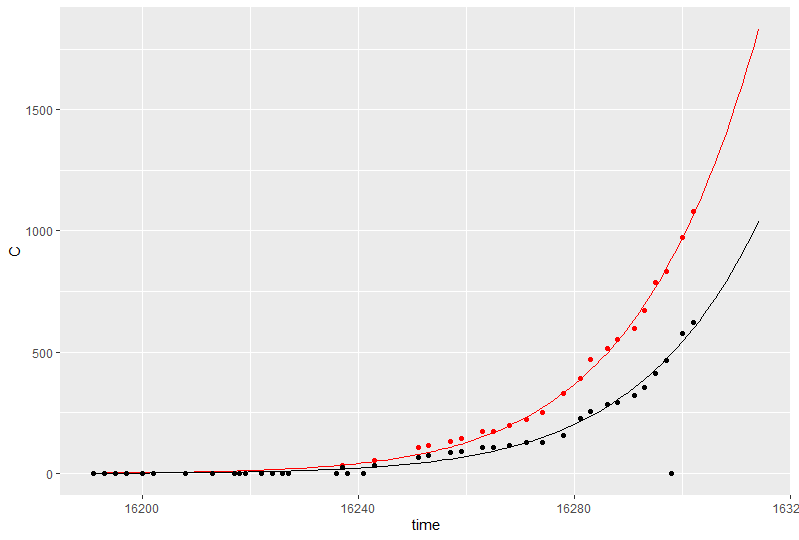
\includegraphics[width=0.7\linewidth]{./figures/my_fit_Lib}
	\caption{Our Liberia Figure}
	\label{fig:my_fit_Lib}
\end{figure}
